\section{Métodos de Deep Learning}
\label{section:metodos}

Nesta seção, explicamos sobre a preparação dos dados e como fizemos o aumento artificial dos dados para obter melhores resultados na avaliação dos modelos. Em seguida, descrevemos as redes convolucionais utilizadas: VGG, Inception Resnet, EfficientNet e DenseNet. Introduzimos o conceito de (\emph{Ensemble}) e descrevemos as técnicas usadas anteriormente e que fundamentaram nossas escolhas. Em seguida, apresentamos as principais definições das redes e parâmetros utilizados neste trabalho e por fim detalhamos como foram feitas as modelagens e treinamentos dos classificadores e do nosso meta-modelo.

\subsection{Preparação dos dados}
\label{section:preparacao}

O pré-processamento é a preparação das imagens para serem usadas pelo modelo, ou seja, é a transformação dos dados não processados em dados prontos para entrada na rede. Isso envolve representar as imagens por matrizes multidimensionais, onde cada elemento da matriz representa um pixel da imagem, e aplicar algumas transformações, especificadas a seguir.

\subsubsection{Agrupamento das bandas para confecção das imagens RGB}

Como as imagens do S-PLUS foram obtidas em 12 bandas fotométricas (listadas em \cite{oliveira2019}), para representá-las no sistema de cor RGB fizemos o seguinte mapeamento: em R colocamos as 4 bandas vermelhas r\_SDSS, i\_SDSS, J0861 e z, em G as bandas g\_SDSS J0515 e J0660 e em B as cinco bandas mais azuis u\_JAVA, J0373, J0395, J0410 e J0430 (as características destes filtros são dadas na Tabela 1 de \cite{oliveira2019}). Na combinação de bandas em cada canal, foi feita uma soma simples dos valores dos píxeis. Depois de reduzidas a três bandas, as imagens são usadas como entrada do programa Trilogy\cite{coe2012clash}\footnote{\url{https://www.stsci.edu/~dcoe/trilogy/Intro.html}}.

\subsubsection{ImageNet}

Como já mostrado em trabalhos anteriores, a inicialização dos pesos provenientes de uma rede pré-treinada usando a base de dados \emph{ImageNet}\footnote{\url{http://www.image-net.org/}} traz uma grande melhoria na precisão dos resultados da classificação. Essa base de dados possui milhões de imagens de objetos do cotidiano e já foi utilizada especificamente para a classificação de objetos astronômicos (veja por exemplo \cite{bom2021}), com excelentes resultados.

O uso deste dataset para pré-treinamento respeitou o pré-processamento utilizado originalmente pelos autores de cada rede, este procedimento este foi crucial para garantir um fit competitivo, isto é, no \textit{benchmarking} original destas redes para os dados da \emph{ImageNet}. Para a rede VGG16 (Seção \ref{section:vgg}), a ordem das bandas foi trocada de RGB para BGR, e cada banda foi centrada em zero em relação à \emph{ImageNet}, sem escalonamento, ou seja, os píxeis de cada banda tiveram o valor da média da respectiva banda \emph{ImageNet} subraído. Para a rede InceptionResNetV2 (Seção \ref{section:inceptionresnetv2}), os píxeis de entrada foram escalonados entre -1 e 1 em relação a amostra de treino. Para a rede EfficientNet (Seção \ref{section:efficientnet}), os píxeis de entrada foram escalonados entre 0 e 1 em relação à amostra de treino. E, para a rede DenseNet (Seção \ref{section:densenet}), os píxeis de entrada foram escalonados entre 0 e 1 e cada banda foi padronizada em relação à \emph{ImageNet}, isto é, os píxeis de cada banda tiveram o valor da média subtraído e o resultado foi dividido pelo desvio padrão da distribuição da respectiva banda da \emph{ImageNet}.


\subsection{Aumento artificial de dados}

\begin{figure*}[!ht]
  \centering
  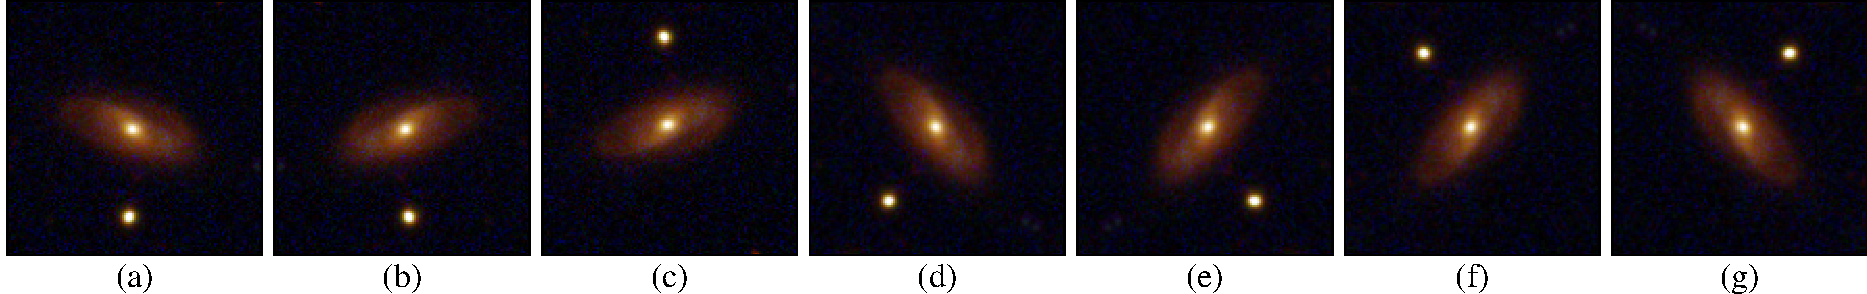
\includegraphics[width=\linewidth]{figures/dataaug.pdf}
  \caption{Exemplo do aumento artificial de dados em uma imagem original, mostrada no painel (a). Os painéis (b), (c), (d), (e), (f) e (g) contêm os resultados da equação \eqref{eq:final-transformation} substituindo $M$ por diferentes combinações das transformações da equação \eqref{eq:transformations}. Em (b) $M = V$, em (c) $M = H$, em (d) $M = R(30\degree)$, em (e) $M = V R(30\degree)$, em (f) $M = H R(30\degree)$ e em (g) $M = H V R(30\degree)$.}
  \label{fig:dataaug}
\end{figure*}

Aumento artificial de dados \cite{Larry1996} é a aplicação de transformações afins nas imagens do conjunto de treinamento, por exemplo rotação, reflexão, translação e mudança de escala. As matrizes da equação \eqref{eq:transformations} definem as transformações usadas.

\begin{equation} \label{eq:transformations}
  \begin{gathered}
    R(\theta) =
    \begin{bmatrix}
      \cos(\theta) & -\sin(\theta) & 0 \\
      \sin(\theta) & \cos(\theta)  & 0 \\
      0            & 0             & 1
    \end{bmatrix}
    \\[1.5ex]
    H =
    \begin{bmatrix}
      1 & 0  & 0 \\
      0 & -1 & 0 \\
      0 & 0  & 1
    \end{bmatrix}
    \quad
    V =
    \begin{bmatrix}
      -1 & 0 & 0 \\
      0  & 1 & 0 \\
      0  & 0 & 1
    \end{bmatrix}
  \end{gathered}
\end{equation}
%
onde $R(\theta)$ é a transformação rotação por um ângulo $\theta$,
$H$ é a transformação reflexão horizontal e $V$ é a transformação reflexão vertical.

Seja $M$ a matriz das transformações combinadas, $(x, y)$ a coordenada do píxel da imagem original e $(x^*, y^*)$ a coordenada transformada do píxel, as transformações nas imagens são feitas remapeando as coordenadas dos píxeis originais aplicando uma combinação das matrizes da equação \eqref{eq:transformations} em cada píxel da imagem original usando a equação \eqref{eq:final-transformation}, onde $(t_x, t_y)$ é a coordenada do centro da imagem e as matrizes ao redor de $M$ são as matrizes translação. Isso é feito para que a transformação $M$ tenha o centro da imagem como ponto de simetria.

\begin{align} \label{eq:final-transformation}
  \begin{bmatrix}
    x^* \\
    y^* \\
    1
  \end{bmatrix}
  =
  \begin{bmatrix}
    1 & 0 & t_x \\
    0 & 1 & t_y \\
    0 & 0 & 1
  \end{bmatrix}
  \ M\
  \begin{bmatrix}
    1 & 0 & -t_x \\
    0 & 1 & -t_y \\
    0 & 0 & 1
  \end{bmatrix}
  \begin{bmatrix}
    x \\
    y \\
    1
  \end{bmatrix}
\end{align}

Além disso, ainda é aplicada uma interpolação bilinear como \emph{anti-aliasing} \cite{aliasing, bilinear}. Durante o treinamento da rede, novas imagens de entrada são geradas a cada época a partir da transformação das imagens originais. A Figura \ref{fig:dataaug} mostra a imagem original, no painel (a), e diversas transformações, nos demais painéis, aplicadas substituindo $M$ da equação \eqref{eq:final-transformation} por combinações (multiplicação matricial) das transformações da equação \eqref{eq:transformations}. Tais transformações não mudam a interpretação da classe da imagem original, pois o espaço visual é invariante a elas. Logo, o objetivo de aplicar estas transformações nas imagens de entrada da rede é deixar que o algorítmo infira tal invariância, criando, assim, uma ``noção'' do espaço visual, o que resulta no aumento do potencial de generalização da rede \cite{Simard2003, CholletBook}. Frequentemente são relatados bons resultados com o uso desta técnica \cite{EfficientNetEx01, EfficientNetEx02, CNNEx04}, principalmente quando existe grande similaridade entre as classes.


\subsection{VGG}
\label{section:vgg}
A arquitetura VGG \cite{VGG16} foi criada durante a competição de classificação de imagens \textit{Large Scale Visual Recognition Challenge} \cite{ILSVRC15}. Ela se destaca por estar entre as primeiras redes a adotar, com sucesso, o escalamento em profundidade (quantidade de camadas) para aumentar o desempenho na classificação de imagens usando redes convolucionais. Ela já foi usada em diversas tarefas de classificação, como a classificação de software malicioso \cite{VGG16Ex01}, de plantas \cite{VGG16Ex02} e de tumores cerebrais \cite{VGG16Ex03}.

\subsection{InceptionResNetV2}
\label{section:inceptionresnetv2}
A arquitetura InceptionResNetV2 \cite{InceptionResNetv2} usa os blocos Inception, que são convoluções fatorizadas, introduzidos em \cite{Inception}, motivada pela construção de redes mais profundas com um menor custo computacional e menor overfitting, com a adição de conexões residuais \cite{ResNet} motivada pelo problema de dissipação do Gradiente (\textit{vanishing gradients}). Isso permite treinar redes profundas com maior acurácia e mais rápido. Esta arquitetura já foi usada, por exemplo, para classificação de imagens de satélite \cite{InceptionResNetV2Ex01}, de ultrasonografia \cite{InceptionResNetV2Ex02} e de células cancerígenas \cite{InceptionResNetV2Ex03}.

\subsection{EfficientNet}
\label{section:efficientnet}
A arquitetura EfficientNet \cite{EfficientNet} foi desenvolvida como uma resposta à questão de como escalar modelos de convolução. Foram considerados três diferentes aspectos: profundidade, largura e resolução da imagem de entrada. Em vez de dimensionar cada aspecto manualmente, o modelo implementa um escalonamento composto que equilibra os aspectos para obter melhor desempenho, com isso a rede consegue uma alta acurácia usando muito menos parâmtros e operações de ponto flutuante por segundo (\emph{FLOPS}). Esta rede já foi usada na classificação de doenças em vegetais \cite{EfficientNetEx03}, eletrocardiogramas \cite{EfficientNetEx01} e cristalização de proteínas \cite{EfficientNetEx02}.

\subsection{DenseNet}
\label{section:densenet}
A rede DenseNet \cite{DenseNet} também usa conexões residuais que conectam cada camada a todas as outras camadas seguintes, o que reduz ainda mais o número de parâmetros na rede sem perda significativa da precisão. O uso desta rede incluem predição do mapa de contato de proteínas \cite{DenseNetEx02}, classificação de músicas \cite{DenseNetEx05}, câncer de mama \cite{DenseNetEx01} e esclerose múltipla \cite{DenseNetEx03}.

\subsection{Ensemble}

\begin{figure*}[!ht]
  \centering
  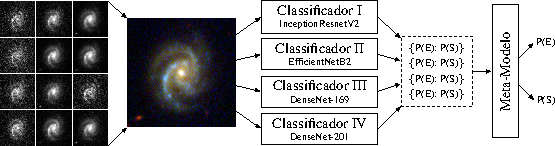
\includegraphics[width=\textwidth]{figures/arch.pdf}
  \caption{Diagrama que descreve a arquitetura da rede. Da esquerda para a direita, as 12 imagens de cada banda são agrupadas em uma única imagem RGB (Seção \ref{section:preparacao}), que é a entrada dos classificadores indidviduais. Estes classificadores (Seção \ref{section:classificador}) têm a função de extrair características visuais da imagem e retornar a probabilidade de ser elíptica ou espiral. O meta-modelo (Seção \ref{section:meta-modelo}) tem a função de combinar as predições dos classificadores em uma única predição final mais robusta.}
  \label{fig:arch}
\end{figure*}

Abaixo mostraremos como podemos combinar os resultados das redes descritas na última seção, usando um método de  \emph{Ensemble}, que combina os vários modelos treinados para resolver um mesmo problema. Essse ensemble foi feito inspirado em \cite{Frayman2002}, que mostraram uma grande melhoria nos resultados quando várias redes são combinadas numa regressão logística. O uso de \emph{Ensemble} tem se mostrado uma importante técnica no desenvolvimento de modelos de \emph{machine learning} ainda nos anos 90, quando Hansen \& Salamon \cite{Hansen1990} mostraram que as predições feitas pela combinação de um conjunto de classificadores são frequentemente mais precisas do que as feitas somente pelo melhor classificador. Existem vários relatos de sucesso do uso desta técnica em \emph{deep learning}, dentre eles a classificação de retina humana \cite{EnsembleEx01}, melanoma \cite{EnsembleEx02} e de anomalias na Via Láctea \cite{EnsembleEx03}. Existem várias técnicas de agrupamento (\emph{Ensemble}), como \emph{Boosting} \cite{Kearns1989, Schapire1990}, \emph{Bagging} \cite{Breiman1996} e \emph{Stacking} \cite{Wolpert1992, Breiman1996b, Smyth1999}.
Este último foi o escolhido para ser usado neste trabalho. Ele se diferencia dos demais pela presença de um meta-modelo, que recebe as predições dos classificadores -- treinados individualmente -- e retorna uma predição final, como é mostrado na Figura \ref{fig:arch}.
A Figura \ref{fig:arch} mostra a arquitetura do \emph{Ensemble} a partir do processo de inferência de uma imagem. Pelo diagrama, é possível notar que o modelo é composto de duas camadas de redes neurais artificiais, a primeira é composta pelos classificadores e a segunda é composta pelo meta-modelo. As Seções \ref{section:classificador} e \ref{section:meta-modelo} detalham o desenvolvimento da primeira e segunda camadas respectivamente.

Uma outra etapa importante no desenvolvimento de redes neurais artificiais é o ajuste dos hiper-parâmetros, alguns deles mostrados na Seção \ref{section:hyperparam}.

\subsection{Definições das redes e parâmetros utilizados}
\label{section:hyperparam}

Nesta seção descrevemos as definições dos principais conceitos, no contexto de deep learning, que serão úteis para o entendimento dos métodos aqui utilizados. A função de ativação, função de custo, o otimizador, o learning rate, o número de épocas, além do número de camadas dos modelos, são importantes parâmetros responsáveis pela contrução do modelo definido a seguir.

\begin{description}
  \item[Função de ativação] \hfill \\
        A função de ativação é responsável por adicionar não-linearidade à rede. Sem ela, a saída de uma camada seria apenas uma transformação linear dos dados de entrada e a rede não seria beneficiada pelo empilhamento de diversas camadas lineares, pois isso não aumentaria o espaço de hipóteses. Logo, a função de ativação viabiliza representações mais complexas da rede, uma vez que define a complexidade de um modelo e, consequentemente, sua capacidade de generalização \cite{CholletBook}. Neste trabalho, a função $\rm{ReLU}(x) := \rm{max}(0, x)$ é usada nas camadas densas dos classificadores, a equação tangente hiperbólica é usada nas camadas densas do meta-modelo e a função Softmax \cite{Bridle1990} foi usada na última camada, tanto dos classificadores quanto do meta-modelo.

  \item[Função de Custo] \hfill \\
        A função de custo é utilizada com o objetivo de determinar o quão longe o modelo está do esperado, definindo a necessidade de atualização dos pesos da rede. Utilizamos a função Entropia Cruzada (\emph{Cross-Entropy})
        \begin{equation}
          \label{eq:custo}
          J = \sum_{i=1}^{C} y_i \cdot \rm{log}(\hat{y}_i)
        \end{equation}
        onde $y_i$ representa a probabilidade da classe dada pelo conjunto de treinamento do objeto $i$ e $\hat{y}_i$ representa a previsão da rede para este mesmo objeto.

  \item[Otimizador] \hfill \\
        O otimizador é um algorítmo iterativo com objetivo de minimizar a função de custo. Uma escolha típica é o método de gradiente descente e suas demais variações. Este tipo de algoritmo tem um parâmetro livre relacionado ao passo da iteração conhecido como taxa de aprendizado ou \textit{learning rate}. Neste trabalho foram testados diversos algoritmos considerados como estado-da-arte dos otimizadores como Adam \cite{Adam}, NAdam \cite{NAdam}, RAdam \cite{RAdam} e RMSprop \cite{RMSprop}.

  \item[Número de Épocas] \hfill \\
        O Número de épocas se referem a quantidade de vezes que o dataset de treino foi utilizado completamente no processo de otimização iterativa da função de custo. Um número de épocas adequado é necessário para que a função de custo seja minimizada.

  \item[Tamanho do Batch] \hfill \\
        O processo de otimização acontece em batches, cada iteração para minimizar a função custo é realizada com um número fixo de amostras, quando todas as amostras de treino são utilizadas se completa uma época.

  \item[Unidades de neurônios na última camada]
        \hfill \\
        A última camada da rede antes da camada de saída é responsável por condensar toda a informação extraída da rede para o processo de classificação final. Por esta razão, a quantidade de neurônios nessa camada pode ser particularmente sensível para a performance da rede. Neste trabalho utilizamos diferentes valores de neurônios para encontrar a quantidade que pode gerar a melhor performance.

  \item[Dropout]
        \hfill \\
        \emph{Dropout} \cite{dropout} é uma técnica de regularização muito utilizada em redes neurais por seu bom desempenho e baixo custo computacional. Aplicar esta regularização em uma camada consiste em eliminar aleatoriamente uma taxa dos neurônios de saída desta camada durante o treinamento, sendo geralmente escolhido um valor entre 0.2 e 0.5 para esta taxa \cite{CholletBook}.
\end{description}

\subsection{Modelagem e Treinamento dos Classificadores}
\label{section:classificador}

\begin{table}[!ht]
  \centering
  \caption{Variação dos parâmetros dos classificadores com arquitetura InceptionResNetV2 usando \emph{oversample}.}
  \label{tab:First_step_hip}
  \doubleRuleSep
  \begin{tabular}{l*{3}{r}}
    \doubleTopRule
    Parâmetro                          & Valor             & ROC AUC       & PR AUC        \\
    \midrule
    \multirow{4}{*}{Otimizador}        & Adam              & 0.983551      & 0.984164      \\
                                       & RAdam             & 0.981333      & 0.982089      \\
                                       & NAdam             & \bf{0.985507} & \bf{0.986090} \\
                                       & RMSprop           & 0.976397      & 0.977327      \\
    \midrule[0.3pt]
    \multirow{7}{*}{\shortstack{\emph{Learning}                                            \\\emph{Rate}}} & $5 \cdot 10^{-6}$ & 0.970411 & 0.971590 \\
                                       & $1 \cdot 10^{-5}$ & 0.978090      & 0.978931      \\
                                       & $5 \cdot 10^{-5}$ & \bf{0.986820} & \bf{0.987339} \\
                                       & $1 \cdot 10^{-4}$ & 0.986380      & 0.986919      \\
                                       & $5 \cdot 10^{-4}$ & 0.985809      & 0.986337      \\
                                       & $1 \cdot 10^{-3}$ & 0.981214      & 0.979992      \\
                                       & $5 \cdot 10^{-3}$ & 0.977913      & 0.976907      \\
    \midrule[0.3pt]
    \multirow{5}{*}{\emph{Batch Size}} & 32                & 0.974966      & 0.972293      \\
                                       & 64                & 0.981530      & 0.980156      \\
                                       & 128               & 0.976305      & 0.974936      \\
                                       & 192               & \bf{0.985100} & \bf{0.985659} \\
                                       & 256               & 0.983728      & 0.984385      \\
    \midrule[0.3pt]
    \multirow{6}{*}{Unidades}          & 128/2             & 0.977434      & 0.978307      \\
                                       & 256/2             & 0.979423      & 0.980226      \\
                                       & 512/2             & \bf{0.986420} & \bf{0.986917} \\
                                       & 1024/2            & 0.981792      & 0.982526      \\
                                       & 256/128/2         & 0.979862      & 0.980575      \\
                                       & 1024/256/128/2    & 0.982252      & 0.982909      \\
    \doubleBottomRule
  \end{tabular}
\end{table}

A estrutura de cada classificador é composta por um extrator de características ligado a um bloco de camadas densamente conectadas, também chamado de bloco de predição. O extrator de características é uma rede neural convolucional usada como camada de abstração das características visuais, detectando padrões como geometrias, contrastes, texturas e cores na imagem de entrada. Enquanto que o bloco de predição recebe estas característcas e retornam as probabilidades da imagem pertencer à classe elíptica e espiral.

Para o extrator de características, foram testadas arquiteturas conhecidas de redes convolucionais descritas anteriormente: InceptionResNet, EfficientNet, DenseNet e VGG. Cada uma destas arquiteturas foi pré-treinada usando a base de dados \emph{ImageNet}.

Para as camadas densas, foram testadas várias configurações de escalamento, tanto em largura (quantidade de neurônios) quanto em profundidade (quantidade de camadas). As configurações testadas consistem de $m$ camadas ocultas com $n$ unidades de neurônios ($m$ variando de 0 a 3 e $n = 2^t$, com $t$ variando de 6 a 10) ligadas a uma camada final com 2 unidades de neurônios e função de ativação \emph{Softmax}. Cada unidade desta última camada representa a probabilidade do objeto pertencer a cada classe \cite{Goodfellow2016}, i.e., elíptica e espiral. Por isso o número de neurônios é igual ao número de classes e suas configurações não foram variadas.

Além disso, as camadas ocultas foram regularizadas com \emph{dropout}, que garante uma melhora na capacidade de generalização da rede \cite{dropout2}. A avaliação dos modelos nos conjuntos de treinamento e de validação mostraram que a melhor taxa de \emph{dropout} é $0.4$, superando a avalição das redes sem regularizador e das redes com outras taxas de \emph{dropout} no intervalo entre 0.1 e 0.6. Do mesmo modo, a função de ativação \emph{ReLU} garantiu as melhores avaliações dos modelos quando comparadas com outras funções de ativação, como tanh e \emph{ELU}.


Outras configurações da rede também foram testadas, tanto relacionadas aos dados, como a amostragem, quanto relacionadas ao treinamento, como o tamanho do \emph{batch}, o algorítmo de otimização e a sua taxa de aprendizagem. Com a variação de um parâmetro por vez, é possível detectar os valores que contribuem para a melhor avaliação da rede, como visto na Tabela \ref{tab:First_step_hip}. Nesta tabela, é mostrado que um modelo treinado usando o otimizador NAdam com uma taxa de aprendizagem de $5 \cdot 10^{-5}$ e 192 exemplares por \emph{batch}, além de um bloco de predição contendo uma camada de 512 unidades de neurônios seguida de uma camada com 2 unidades, obteve a melhor avaliação no conjunto de validação em relação às outras configurações. Isso mostra como foram determinados os parâmetros do Modelo A da Tabela \ref{tab:best_hip}, mostrada na Seção \ref{section:resultados}. Os parâmetros para os demais modelos foram obtidos analogamente.




\subsection{Modelagem e Treinamento do Meta-Modelo}
\label{section:meta-modelo}

O objetivo do meta-modelo é receber as predições de cada um dos classificadores e retornar uma predição final. Para isso, foi usada uma rede neural com estrutura composta por uma camada de entrada de 8 unidades de neurônios seguidas de duas camadas ocultas de 128 unidades e uma camada de saída com 2 unidades. Assim como nos classificadores, diversas configurações de hiperparâmetros foram testadas para o meta-modelo. Sendo que a configuração que gerou o melhor resultado na avaliação foi usando a função de ativação tangente hiperbólica nas camadas ocultas, \emph{batch size} de 32 e o otimizador Adam com uma taxa da aprendizagem de $1 \cdot 10^{-5}$.

Como a entrada do meta-modelo são as predições dos classificadores, o conjunto de treinamento deve ser gerado a partir destes valores. Sendo assim, para criação do conjunto de treinamento do meta-modelo, foi usado um processo iterativo chamado validação cruzada k-fold (\emph{k-fold cross-validation}). Neste método, o conjunto de treinamento é dividido em $k$ amsotras de mesmo tamanho, sendo uma delas usada obter as predições enquanto as $k-1$ restantes são usadas como treino. O processo se repete por $k$ vezes, variando a amostra usada para predição. No final da repetição deste processo para cada classificador, é obtido um conjunto de treinamento para o meta-modelo do mesmo tamanho do conjunto de treinamento original, com a vantagem que as predições foram feitas em uma amostra não usada no treinamento. Para o treinamento deste meta-modelo, foi usado um valor de $k=5$.

Para reduzir o impacto da variância das predições do conjunto de treinamento na predição final do meta-modelo, o valor usado como entrada do meta-modelo foi a mediana de 12 repetições da validação cruzada feitas para cada um dos classificadores. Além disso, os dados de entrada ainda receberam um pré-processamento, eles foram subtraídos da média e divididos pelo desvio padrão em relação às predições de cada classificador. Ao contrário dos classificadores, as camadas ocultas do meta-modelo não foram regularizadas com \emph{dropout}.
